\documentclass{scrartcl}

\usepackage{graphicx}
\usepackage[utf8]{inputenc}
\usepackage[T1]{fontenc}
\usepackage{lmodern}
\usepackage[english]{babel}
\usepackage{amsmath}
\usepackage{amsthm}
\usepackage{mathtools}
\usepackage{amssymb}
\usepackage{listings}
\usepackage{xparse}
\usepackage{geometry}
\usepackage{hyperref}
\usepackage{enumerate}
\usepackage{tikz}
\usepackage[style=english]{csquotes}
\usepackage[language=english, backend=biber, style=alphabetic, sorting=nyt]{biblatex}

\usetikzlibrary{babel, positioning, shapes.geometric, arrows, arrows.meta}
\addbibresource{bibliography.bib}

\title{Some Notes on Algebraic Maps, Elliptic Curves and Isogenies}
\author{Simon Pohmann}

\hypersetup{
    colorlinks,
    linkcolor={red!50!black},
    citecolor={blue!50!black},
    urlcolor={blue!80!black}
}

\newcommand{\N}{\mathbb{N}}
\newcommand{\Z}{\mathbb{Z}}
\newcommand{\F}{\mathbb{F}}
\newcommand{\I}{\mathbb{I}}
\newcommand{\V}{\mathbb{V}}
\newcommand{\C}{\mathbb{C}}
\newcommand{\Aff}{\mathbb{A}}
\newcommand{\Proj}{\mathbb{P}}
\newcommand{\Half}{\mathcal{H}}
\newcommand{\SL}{\mathrm{SL}}
\newcommand{\End}{\mathrm{End}}
\newcommand{\Ell}{\mathrm{Ell}}
\newcommand{\Quot}{\mathrm{Quot}}
\newcommand{\Cl}{\mathrm{Cl}}
\renewcommand{\O}{O}
\newcommand{\Order}{\mathcal{O}}
\newcommand{\divides}{\ \mid \ }
\newcommand{\notdivides}{\ \nmid \ }

\newcommand\restr[2]{{
    \left.\kern-\nulldelimiterspace
    #1
    \vphantom{\big|}
    \right|_{#2}
}}

\newtheorem{prop}{Proposition}[section]
\newtheorem{theorem}[prop]{Theorem}
\newtheorem{lemma}[prop]{Lemma}
\newtheorem{corollary}[prop]{Corollary}

\theoremstyle{definition}
\newtheorem{problem}[prop]{Problem}
\newtheorem{alg}[prop]{Algorithm}
\newtheorem{definition}[prop]{Definition}
\newtheorem{example}[prop]{Example}
\newtheorem{remark}[prop]{Remark}

\begin{document}

\maketitle

\tableofcontents

\section{Maps on varieties}

\subsection{Algebraic maps}
First of all, we define the basic notions of algebraic maps, that is maps that are locally defined by polynomials.
For simplicity of notation, we already introduce the projective coordinate ring before.
\begin{definition}
    Let $X \subseteq \Proj^n$ be a projective variety. 
    Then the graded ring $S(X) := k[x_0, ..., x_n] / \I(X)$ is its projective coordinate ring.
\end{definition}
Note that the graded ring is not invariant under isomorphisms of projective varieties.
\begin{definition}
    Let $X \subseteq \Proj^n$ and $Y \subseteq \Proj^m$ be quasi-projective varieties, i.e. open subsets of the projective varieties $\bar{X}, \bar{Y}$.
    Then define
    \begin{itemize}
        \item A map $X \to Y$ is called \emph{morphism}, if it is given locally by polynomials, so for each $p \in X$ there is an open neighborhood $U$ of $p$ and homogeneous polynomials $f_0, ..., f_m \in S(\bar{X})$ of same degree such that
        \begin{equation*}
            (f_0(a), ..., f_m(a)) \neq 0 \ \text{and} \ f(a) = [f_0(a) : ... : f_m(a)] \ \text{for all $a \in U$}
        \end{equation*}
        \item A partial map $X \dashrightarrow Y$ on an irreducible quasi-projective variety $X$ is called \emph{rational}, if its set of definition is an open subset $U \subseteq X$ and it is a morphism $U \to Y$.
        We identify rational maps $f, g: X \dashrightarrow Y$ defined on $U, V \subseteq X$ if $\restr{f}{U \cap V} = \restr{g}{U \cap V}$.
        In other words, rational maps are morphisms $U \to Y$ with maximal domain $U \subseteq X$ open.
    \end{itemize}
\end{definition}
In particular, morphisms and rational maps are technically the same thing.
The definitions just differ in the domain, not in the key property ``locally defined by polynomials''.
This distinction is mostly an artifact of the definition of varieties via vanishing loci, and is no longer necessary when one uses the ``modern'' approach to algebraic geometry based on schemes.

\subsection{The coordinate rings}
We have already introduced the projective coordinate ring, which is a not totally natural object, because it is not invariant under isomorphisms.
Affine varieties have a much nicer coordinate ring.
\begin{definition}
    For an affine variety $X \subseteq \Aff^n$, define the affine coordinate ring $k[X] := k[x_1, ..., x_n] / \I(X)$.
\end{definition}
This ring has a much tighter connection to the variety.
\begin{theorem}
    \label{prop:equivalence_of_categories}
    Let $\mathcal{V}$ be the category of affine varieties $\subseteq \Aff_k^n$ with affine morphisms, and $\mathcal{A}$ the category of finitely generated, reduced (commutative, unital) $k$-algebras.
    Then
    \begin{align*}
        \Phi: \mathcal{V}^{\mathrm{op}} \to \mathcal{A}, \quad V \mapsto k[V], \ \phi \mapsto \phi^*
    \end{align*}
    is an equivalence of categories.
\end{theorem}
Further, each irreducible affine and projective (and even quasi-projective) variety has a function field.
\begin{definition}
    For an irreducible affine variety $X \subseteq \Aff^n$, define the \emph{function field} as the field of fractions $k(X) := \mathrm{Frac}(k[X])$.
    For an irreducible projective variety $X \subseteq \Proj^n$, define the \emph{function field} as
    \begin{equation*}
        k(X) := \left\{ f/g \in \mathrm{Frac}(S(X)) \ \middle| \ f, g \ \text{homogeneous polynomials of same degree} \right\}
    \end{equation*}
\end{definition}
Note that we can evaluate an element $\frac f g \in k(X)$ at all points $a \in X \setminus \V(g)$ and get a well-defined value in $k$.
To get the function field of an arbitrary quasi-projective variety, one can define it as the function field of an affine chart.
We will not pursue that path further.
However, the following lemma is important.
\begin{lemma}
    Let $X \subseteq \Proj^n$ be an irreducible projective variety. Then for all embeddings $\Aff^n \subseteq \Proj^n$ get
    \begin{equation*}
        k(X \cap \Aff^n) \cong k(X) \quad \text{via} \quad \frac f g \mapsto \frac {x_0^d f({x_1} / {x_0}, ..., {x_n} / {x_0})} {x_0^d g({x_1} / {x_0}, ..., {x_n} / {x_0})}, \ d = \max \{\deg f, \deg g\}
    \end{equation*}
    Further, find that $k(X)$ is invariant under isomorphisms.
    If the embedding $\Aff^n \subseteq \Proj^n$ is clear, we will sometimes identify both fields.
\end{lemma}
Hence, the function field is again a natural property of varieties.

\subsection{Describing rational maps}
The function field is more or less equal to all regular maps defined on \emph{some} open subset of $X$. Namely
\begin{prop}
    Let $X \subseteq \Proj^n$ be an irreducible projective variety.
    Have a well-defined and injective $k$-algebra homomorphism
    \begin{equation*}
        \mathcal{O}_X(U) \to k(X), \quad f: U \to k \ \text{defined locally at $p \in U$ by $f = g/h$} \ \mapsto \ \frac g h
    \end{equation*}
    Further, this is in some sense surjective, meaning that for each $f \in k(X)$ there is some open $U \subseteq X$ such that $f$ is contained in the image of $\mathcal{O}_X(U) \to k(X)$.
\end{prop}
If we only consider regular maps that are defined on the whole of $X$, we get the following statement.
\begin{theorem}
    If $X \subseteq \Proj^n$ is a projective variety, find $\mathcal{O}_X(X) \cong k$.
    If $X \subseteq \Aff^n$ is an affine variety, find $\mathcal{O}_X(X) \cong k[X]$.
\end{theorem}
\begin{proof}
    Consider the map
    \begin{equation*}
        k[X] \to \mathcal{O}_X(X), \quad f \mapsto (a \mapsto f(a))
    \end{equation*}
    which is clearly a well-defined, injective $k$-algebra homomorphism.
    So for the second part, it is left to show that it is surjective.

    Let $f \in \mathcal{O}_X(X)$.
    Then for each $p \in X$ there is an open neighborhood $U_p \subseteq X$ and polynomials $g_p, h_p \in S(X)$ with $f = g_p/h_p$ on $U_p$ with $h_p(a) \neq 0$ for all $a \in U_p$.
    As $X \subseteq \Aff^n$, we can assume $g_p, h_p \in k[X]$.
    Obviously, there is a finite subcover $U_1 := U_{p_1}, ..., U_r := U_{p_r}$ with $p_1, ..., p_r \in X$.

    As the $U_i$ are an open cover, we see that $\V(\langle h_1, ..., h_r \rangle) = \emptyset$ and so by Hilbert's Nullstellensatz, find
    \begin{equation*}
        1 = \sum_i \alpha_i h_i
    \end{equation*}
    Thus
    \begin{equation*}
        f_i := \frac {g_i} {h_i} = \frac {g_i} {h_i} \sum_j \alpha_j h_j = \alpha_i g_i + \sum_{j \neq i} \alpha_j h_j \in k[X] \subseteq k(X)
    \end{equation*}
    So on each $U_i$, the regular map $f$ is given by a polynomial $f_i \in k[X]$.
    It is left to show that those glue together to one global polynomial (this is only trivial in the case $X$ irreducible).
\end{proof}
Describing rational maps and morphisms can be done similarly, but they also allow a relatively nice definition using the function field.
\begin{theorem}
    \label{prop:rational_map_function_field}
    Let $X \subseteq \Proj^n$ be an irreducible projective variety. Then there is a well-defined bijection
    \begin{align*}
        \Phi: \{ f: X \dashrightarrow \Proj^m \ | \ f \ \text{rational map} \} &\to \Proj_{k(X)}^m, \\
        f \ \text{defined locally by $f_0, ..., f_m \in S(X)$} &\mapsto \left[ \frac {f_0} {x_0^d}  : \frac {f_1} {x_0^d} : ... : \frac {f_n} {x_0^d} \right]
    \end{align*}
    In particular, the restriction
    \begin{equation*}
        \restr{\Phi}{\{f: X \to \Proj^m \ | \ f \ \text{morphism}\}}: \{f: X \to \Proj^m \ | \ f \ \text{morphism}\} \to \Proj_{k(X)}^m
    \end{equation*}
    is a well-defined injection.
\end{theorem}
We sometimes will identify those two representations of rational maps.
Note that $k[X \cap \Aff^n] \subseteq k(X \cap \Aff^n) \cong k(X)$, and using this makes the notation of rational maps as $[f_0 : ... : f_m]$ even more convenient, because we do not even require fractions then.

Furthermore, the rational maps $X \dashrightarrow Y$ to a projective variety $Y$ are then exactly the elements of 
\begin{equation*}
    \V_{k(X)}(\I_k(Y)) \subseteq \Proj^m_{k(X)}
\end{equation*}
and similarly for open sets.

\begin{remark}
    Note that the bijection $\Phi$ from Theorem~\ref{prop:rational_map_function_field} is compatible with evaluation maps in the following sense.
    For $f: X \dashrightarrow Y$ and $g: Y \dashrightarrow \Proj^r$ such that the composition $g \circ f$ is well-defined, have
    \begin{equation*}
        \Phi(g \circ f) = \mathrm{ev}_{\Phi(f)}(\Phi(g))
    \end{equation*}
\end{remark}

\begin{definition}
    Let $f = [f_0 : ... : f_m]: X \dashrightarrow Y$ be a rational map with $f_0, ..., f_m \in k(X)$.
    Then
    \begin{equation*}
        f^*: k(Y) \to k(X), \quad y_i \mapsto f_i
    \end{equation*}
    is called the \emph{pullback} of $f$.
\end{definition}

\section{Elliptic Curves}

\begin{definition}[Elliptic Curve]
    An elliptic curve $E \subseteq \Proj^2$ is a nonsingular curve given by an equation of the form
    \begin{equation*}
        E = \V( Y^2 Z + a_1 XYZ + a_3 YZ^2 - X^3 - a_2 X^2 Z - a_4 XZ^2 - a_6 Z^3 )
    \end{equation*}
    We write $\O := [0 : 1 : 0]$ for the unique point of $E$ on the hyperplane at infinity.
    Further, write $k[E]$ for the affine coordinate ring $k[E \cap \Aff^2]$.
\end{definition}

We will often use dehomogenized equations to specify an elliptic curve.

\begin{definition}[Isogeny]
    An isogeny $f: E \to E'$ between elliptic curves is a morphism with $f(\O) = \O$.
    An isogeny that is an isomorphisms in the sense of Algebraic Geometry is also called isomorphism.
\end{definition}

\begin{prop}
    \label{prop:isogeny_surjective}
    Let $f: E \to E'$ be a nonconstant isogeny. 
    Then $f$ is surjective.
\end{prop}
\begin{proof}
    It is a fact from Algebraic Geometry that the image of a projective variety under a morphism is a projective variety.
    So the image of $f$ must be an irreducible projective subvariety of $E'$, hence either a single point or $E'$.
\end{proof}

\begin{prop}
    If $\mathrm{char}(k) \neq 2, 3$ then each elliptic curve is isomorphic to an elliptic curve of the form
    \begin{equation*}
        y^2 = x^3 + A x + B
    \end{equation*}
\end{prop}

\begin{definition}[Discriminant]
    For an elliptic curve $E: y^2 + a_1 xy + a_3 y = x^3 + a_2 x^2 + a_4 x + a_6$, define the discriminant
    \begin{align*}
        \Delta(E) = & - b_2^2 b_8 - 8 b_4^3 - 27 b_6^2 + 9 b_2 b_4 b_6 \\
        \text{where} \quad & b_2 = a_1^2 + 4 a_2 \\
        & b_4 = a_1 a_3 + 2 a_4 \\
        & b_6 = a_3^2 + 4 a_6 \\
        & b_8 = a_1^2 a_6 + 4 a_2 a_6 - a_1 a_3 a_4 + a_2 a_3^2 - a_4^2
    \end{align*}
\end{definition}

Note that for elliptic curves $E$ given by the simpler equation $E: y^2 = x^3 + Ax + B$ have
\begin{equation*}
    \Delta(E) = -16(4A^3 - 27B^2)
\end{equation*}

\begin{prop}
    A cubic curve
    \begin{equation*}
        C = \V( Y^2 Z + a_1 XYZ + a_3 YZ^2 - X^3 - a_2 X^2 Z - a_4 XZ^2 - a_6 Z^3 )
    \end{equation*}
    is an elliptic curve (i.e. nonsingular), if and only if $\Delta(C) \neq 0$.
\end{prop}

\begin{lemma}
    \label{prop:morphism_depends_on_y}
    Let $\psi = [\psi_0, \psi_1, 1]: E \to E'$ be a morphism between elliptic curves.
    Then $k(\psi_0, \psi_1, x) = k(x, y)$.
\end{lemma}
\begin{proof}
    Assume that we have $E': y^2 = x^3 + Ax + B$.
    Then clearly
    \begin{equation*}
        \psi_1^2 = \psi_0^3 + A\psi_0 + B
    \end{equation*}
    Now assume for a contradiction that $\psi_0, \psi_1 \in k(x)$.
    Since $k$ is algebraically closed, have $x^3 + Ax + B = (x - \mu_1)(x - \mu_2)(x - \mu_3)$ and so
    \begin{equation*}
        (\psi_0 - \mu_1)(\psi_0 - \mu_2)(\psi_0 - \mu_3)
    \end{equation*}
    is a perfect square in $k(x)$.
    Note that $\Delta(E')$ is a constant multiple of the discriminant of the polynomial $x^3 + Ax + B$ and since $\Delta(E') \neq 0$, we see that $\mu_1, \mu_2, \mu_3$ are pairwise distinct.
    With $\phi_0 = f/g$ and $f, g \in k[x], f \perp g$ we see that then the factors $f - \mu_1 g, f - \mu_2 g$ and $f - \mu_3 g$ are pairwise coprime, so each must already be a perfect square, say
    \begin{equation*}
        f - \mu_1 g = h_1^2, \ f - \mu_2 g = h_2^2, \ f - \mu_3 g = h_3^2
    \end{equation*}
    with pairwise coprime $h_1, h_2, h_3$. Then
    \begin{align*}
        &(\mu_2 - \mu_1) g = (h_1 - h_2)(h_1 + h_2), \\
        &(\mu_3 - \mu_1) g = (h_1 - h_3)(h_1 + h_3)
    \end{align*}
    Since $h_2 \perp h_3$, find $(h_1 + h_2) \perp (h_1 + h_3)$ and $(h_1 - h_2) \perp (h_1 - h_3)$, so
    \begin{equation*}
        h_1 - h_2 = \epsilon(h_1 + h_3), \ h_1 + h_2 = \epsilon'(h_1 - h_3)
    \end{equation*}
    for some $\epsilon, \epsilon' \in k^*$. Thus $(1 - \epsilon)h_1 = \epsilon h_3 + h_2$ with $\epsilon - 1 \in k^*$.
    So
    \begin{equation*}
        2h_1 = (\epsilon + \epsilon')h_1 + (\epsilon - \epsilon')h_3
    \end{equation*}
    thus
    \begin{equation*}
        (2 - \epsilon - \epsilon')h_1 = (\epsilon - \epsilon')h_3
    \end{equation*}
    and so $\epsilon = \epsilon' = 1$ since $h_1 \perp h_3$. 
    However then $h_3 = -h_2$, a contradiction.
\end{proof}

\subsection{The group law}

\begin{prop}
    \label{prop:bezout_theorem_case}
    Let $E$ be an elliptic curve. Then each projective line meets $E$ at exactly three points, with multiplicity.
\end{prop}

\begin{definition}
    Define a map
    \begin{equation*}
        +_{\mathrm{geo}}: E \times E \to E
    \end{equation*}
    that for $P, Q \in E$ is given by the following geometric construction:
    \begin{itemize}
        \item Let $L$ be the line through $P, Q$ (with multiplicity)
        \item Let $R$ be the third point of intersection of $E$ with $L$ (exists by \ref{prop:bezout_theorem_case})
        \item Let $L'$ be the line through $R, \O$
        \item Set $P +_{\mathrm{geo}} Q$ to be the third point of intersection of $E$ with $L'$
    \end{itemize}
\end{definition}

\begin{prop}
    \label{prop:dedekind_domain}
    Let $E: y^2 = x^3 + Ax + B$ be an elliptic curve. Then the affine coordinate ring $k[E]$ is a Dedekind domain and there is a bijection
    \begin{equation*}
        \phi: E \to \mathrm{Cl}(k[E]), \quad (\lambda, \mu) \mapsto \overline{\langle x - \lambda, y - \mu \rangle}, \ \O \mapsto \overline{\langle 1 \rangle}
    \end{equation*}
\end{prop}

\begin{definition}
    Define the map
    \begin{equation*}
        +_{\mathrm{alg}}: E \times E \to E, \quad (P, Q) \mapsto  \phi^{-1}(\phi(P) \phi(Q))
    \end{equation*}
\end{definition}

\begin{definition}
    Define the map 
    \begin{align*}
        +_{\mathrm{poly}}: E \times E \to E, \quad ((x_1, y_1), (x_2, y_2)) &\mapsto (x_3, y_3), \\
        ((x, y), (x, -y)) &\mapsto \O \\
        (\O, P), \ (P, \O) &\mapsto P
    \end{align*}
    where for $P = (x_1, y_1), \ Q = (x_2, y_2) \neq (x_1, -y_1)$ we set
    \begin{align*}
        \lambda &:= \begin{cases}
            \frac {y_2 - y_1} {x_2 - x_1} \ \text{if} \ x_1 \neq x_2 \\
            \frac {3 x_1^2 + A} {2 y_1} \ \text{otherwise}
        \end{cases} \\
        x_3 &:= -x_1 - x_2 + \lambda^2 \\
        y_3 &:= -y_1 + \lambda (x_1 - x_3)
    \end{align*}
\end{definition}

\begin{prop}[The group law]
    \label{prop:group_operation}
    Let $E$ be an elliptic curve. Then $+ := +_{\mathrm{geo}} = +_{\mathrm{alg}} = +_{\mathrm{poly}}$.
\end{prop}

\begin{corollary}
    Let $E: Y^2 = X^3 + AX + B$ be an elliptic curve. Then 
    \begin{itemize}
        \item $E$ together with the binary operation $+$ from \ref{prop:group_operation} is a group.
        \item $E$ has neutral element $\O$
        \item $E$ is abelian
        \item for a field tower $k|L|K$, the so-called $L$-rational points $E(L) := E \cap \Proj_L^2 = (E \cap L^2) \cup \{ \O \}$ form a subgroup
    \end{itemize}
\end{corollary}

\begin{prop}
    \label{prop:isogeny_homomorphism}
    Let $E, E': y^2 = x^3 + A'x + B'$ be elliptic curves and $\psi: E \to E'$ an isogeny. Then $\psi$ is a group homomorphisms.
\end{prop}
\begin{proof}
    Wlog assume that $\psi$ is nonconstant.
    Have $\psi = [\psi_1 : \psi_2 : 1]$ with $\psi_1, \psi_2 \in k(E)$ and consider the field homomorphism
    \begin{equation*}
        \psi^*: k(E') \to k(E), \quad \overline{f} \mapsto \overline{f( \psi_1, \psi_2 )}
    \end{equation*}
    This is well-defined, because if $\overline{f} = \overline{g}$ then
    \begin{equation*}
        f(\psi_1, \psi_2) \equiv g(\psi_1, \psi_2) \mod \underbrace{\psi_2^2 - \psi_1^3 + A'\psi_1 + B'}_{= (0)}
    \end{equation*}
    Now we look at the field extension 
    \begin{equation*}
        k(E) = k(x, y) \ | \ \psi^*k(E') = k(\psi_1, \psi_2)
    \end{equation*}
    As $\psi(\O) = \O$ we see that there are homogeneous polynomials $f, g, h \in k[R, S, T]$ of same degree with
    \begin{equation*}
        f(0, 1, 0) = h(0, 1, 0) = 0, \ g(0, 1, 0) = 1, \quad \psi_1 = \frac {f^{\mathrm{deh}}(x, y)} {h^{\mathrm{deh}}(x, y)}, \ \psi_2 = \frac {g^{\mathrm{deh}}(x, y)} {h^{\mathrm{deh}}(x, y)}
    \end{equation*}
    Since $f, h$ are homogeneous of same degree, we see that $f(0, y, 0) = h(0, y, 0) = 0$ for all $y \in k$.
    It follows that $\psi_1 \in k(x)$. 
    Furthermore, if $\psi_1 = f(x)/h(x)$ for $f, h \in k[T]$ we can then assume wlog that $f - \psi_1 h \in \psi^*k(E')[T]$ is the minimal polynomial of $x$ over $\psi^*k(E')$ or over $k(\psi_1)$.

    By \ref{prop:isogeny_surjective} we see that $\psi$ is surjective, so Algebraic Geometry tells us that $\psi^*$ is injective.
    We can then define
    \begin{equation*}
        \psi_* := \left(\psi^*\right)^{-1} \circ N_{k(E) | \psi^*k(E')}: k(E) \to k(E')
    \end{equation*}
    This map is a (multiplicative) group homomorphism, as $\psi^*$ is a field homomorphism and the norm map $N$ is multiplicative.
    Thus it induces a well-defined group homomorphism
    \begin{equation*}
        \overline{\psi_*}: \mathrm{Cl}(k[E]) \to \mathrm{Cl}(k[E']), \quad \overline{I} \mapsto \overline{(\psi_*I)}
    \end{equation*}
    Now we show that the following diagram is commutative and the claim follows by \ref{prop:dedekind_domain} and \ref{prop:group_operation}.
    
    \begin{center}
    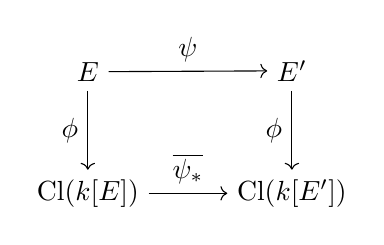
\begin{tikzpicture}
        \node (E) {$E$};
        \node[below = of E] (KE) {$\mathrm{Cl}(k[E])$};
        \node[right = of KE] (KEp) {$\mathrm{Cl}(k[E'])$};
        \node[above = of KEp] (Ep) {$E'$};

        \draw[->] (E) -- (Ep) node[midway, above] {$\psi$};
        \draw[->] (E) -- (KE) node[midway, left] {$\phi$};
        \draw[->] (Ep) -- (KEp) node[midway, left] {$\phi$};
        \draw[->] (KE) -- (KEp) node[midway, above] {$\overline{\psi_*}$};
    \end{tikzpicture}
    \end{center}

    Clearly this holds for $\O$, so consider $(\lambda, \mu) \in E$ with $\psi(\lambda, \mu) \neq \O$.
    As $\psi^*$ is injective, is suffices to show that $(\psi^* \circ \phi \circ \psi)(\lambda, \mu) = (\psi^* \circ \overline{\psi_*} \circ \phi)(\lambda, \mu)$.

    Using the definition of $\phi$ we find
    \begin{align*}
        &(\psi^* \circ \psi_* \circ \phi)(\lambda, \mu) = ( N(x - \lambda), N(y - \mu) ) \quad \text{and} \\
        &(\psi^* \circ \phi \circ \psi)(\lambda, \mu) = \psi^*\left(( x - \psi_1(\lambda, \mu), y - \psi_2(\lambda, \mu) )\right)  = ( \psi_1 - \psi_1(\lambda, \mu), \psi_2 - \psi_2(\lambda, \mu) )
    \end{align*}
    Explicitly computing the determinant of the multiplication map shows that
    \begin{equation*}
        N_{L(\alpha)|L}(\alpha - \lambda) = \mathrm{MiPo}_L(\alpha)(\lambda) \quad \text{so} \quad N(x - \lambda) = \mathrm{MiPo}_{k(\psi_1)}(x)(\lambda)
    \end{equation*}
    By the above, find $f, h \in k[T]$ such that $\psi_1 = f(x)/h(x)$ and $f(T) - \psi_1h(T)$ is the minimal polynomial of $x$.
    Now we see that ($\psi(\lambda, \mu) \neq \O$ so $h(\lambda) \neq 0$)
    \begin{equation*}
        N(x - \lambda) = f(\lambda) - \psi_1h(\lambda) = -h(\lambda)(\psi_1 - \psi_1(\lambda, \mu))
    \end{equation*}
    As $\psi_2^2 = u(\psi_1)$ for some $u \in k[T]$ we find $u, v \in k[S, T]$ such that
    \begin{equation*}
        \mathrm{MiPo}_{\psi^*k(E')}(Y) = v(T, \psi_1)\psi_2 - u(T, \psi_1) \in k(\psi_1, \psi_2)(T)
    \end{equation*}
    Hence
    \begin{equation*}
        N(y - \mu) = v(\mu, \psi_1)\psi_2 - u(\mu, \psi_1)
    \end{equation*}
    As $\mathrm{MiPo}(y)(y) = 0$ have
    \begin{equation*}
        \mathrm{MiPo}(y)(y)(\lambda, \mu) = v(\mu, \psi_1(\lambda, \mu))\psi_2(\lambda, \mu) - u(\mu, \psi_1(\lambda, \mu)) = 0
    \end{equation*}
    Together, modulo $\psi_1 - \psi_1(\lambda, \mu)$ we get
    \footnote{Strictly speaking, we require $v(\mu, \psi_1(\lambda, \mu)) \neq 0$ here, which I haven't considered.
    At least we have $v(y, \psi_1) \neq 0$ here, which follows from Lemma~\ref{prop:morphism_depends_on_y}.}
    \begin{align*}
        \frac 1 {v(\mu, \psi_1(\lambda, \mu))} N(y - \mu) \equiv \psi_2 - \frac {u(\mu, \psi_1)} {v(\mu, \psi_1)} \equiv \psi_2 - \underbrace{\frac {u(\mu, \psi_1(\lambda, \mu))} {v(\mu, \psi_1(\lambda, \mu))}}_{= \psi_2(\lambda, \mu)} = \psi_2 - \psi_2(\lambda, \mu)
    \end{align*}
    So
    \begin{equation*}
        ( N(x - \lambda), N(y - \mu) ) = ( \psi_1 - \psi_1(\lambda, \mu), \psi_2 - \psi_2(\lambda, \mu) ) \in \mathrm{Cl}(k[E])
    \end{equation*}
    and the claim follows.
\end{proof}
\begin{remark}
    In \cite{EllipticCurves}, the above proof was done using the Picard group (which is naturally isomorphic to the ideal class group, but working with it uses different tools).
    Riemann-Roche is not cited (as far as I think) for that proof, but already relies heavily on the theory of divisors.
\end{remark}

Note that the field extension $k(E) | \psi^*k(E')$ is quite important.
In particular, we say
\begin{definition}
    Let $\psi: E \to E'$ be an isogeny.
    We define the \emph{degree} of $\psi$ to be the degree of $k(E) | \psi^*k(E')$ and say that $\psi$ is \emph{separable} if $k(E) | \psi^*k(E')$ is.
\end{definition}

\subsection{Isomorphism classes}

\begin{definition}[j-invariant]
    Let $E: y^2 = x^3 + Ax + B$ be an elliptic curve.
    Then define the j-invariant of $E$ as
    \begin{equation*}
        j(E) := \frac {(-48 A)^3} {\Delta(E)} = 1728 \frac {4A^3} {27 B^2 + 4A^3}
    \end{equation*}
\end{definition}

\begin{prop}
    Let $E, E'$ be two elliptic curves. Then $E \cong E'$ if and only if $j(E) = j(E')$.
\end{prop}
\begin{proof}
    First, assume $j(E) = j(E')$ and consider the isogeny $\psi = [u^2 x, u^3 y, 1]$ where $u^4 = A/A'$.
    Then
    \begin{align*}
        (u^3 y)^2 =& \ u^6 y^2 \quad \text{and} \\
        (u^2 X)^3 - A (u^2 X) - B =& \ u^6 \Bigl(X^3 - \frac 1 {u^4} A X - \frac 1 {u^6} B \Bigr) \\
        =& \ u^6 \Bigl( X^3 - A' X - \frac 1 {u^6} B \Bigr)
    \end{align*}
    From $j(E) = j(E')$ we get
    \begin{equation*}
        A^3 (27 B'^2 + 4A'^3) = A'^3 (27 B^2 + 4A^3)
    \end{equation*}
    Thus
    \begin{equation*}
        A^3 \left( 27 B'^2 + 4\frac 1 {u^{12}} A^3 \right) = \frac 1 {u^{12}} A^3 (27 B^2 + 4A^3)
    \end{equation*}
    and so
    \begin{equation*}
        B'^2 = \frac 1 {u^{12}} B^2 + \frac 1 {27 u^{12}} (4 A^3 - 4 A^3) = \frac 1 {u^{12}} B^2
    \end{equation*}
    It follows that $u^6 = B/B'$ and so $\psi$ maps $E$ to $E'$. 
    It is only a linear transformation, hence also an isomorphism.

    For the other direction, assume there is an isomorphism $\psi = [u, v, 1]$ from $E$ to $E'$ where $E': Y^2 = X^3 + A'X + B'$ and $x, y \in k(E)$.
    As $\psi$ is an isomorphism, it is also an isomorphism of the affine varieties $E \cap \Aff^2$ resp. $E' \cap \Aff^2$ and so we find the pullback
    \begin{equation*}
        \psi^*: k[E'] \to k[E], \quad x' \mapsto u, y' \mapsto v
    \end{equation*}
    for some $u, v \in k[E]$ with $v^2 = u^3 + A'u + B'$
    \footnote{Note that we use a result discussed at the beginning here.
    Namely, the crucial point is that a birational equivalence between affine varieties that is defined everywhere is already an isomorphism.}.
    We want to show that $u, v$ are linear in $x, y \in k[E]$, and the claim follows more or less by reversing the computation above.

    As $\psi$ maps $\O$ to $\O$, we see as before in Prop.~\ref{prop:isogeny_homomorphism} that $u \in k[x]$.
    Since $u$ is transcendental over $k$, we see that $k[x]$ is a finitely generated $k[u]$-module.
    Now we find
    \begin{equation*}
        [k[u] : k[x]] \underbrace{[k[x] : k[x, y]]}_{= 2} = [k[u] : k[x, y]] = \underbrace{[k[u] : k[u, v]]}_{\leq 2} \underbrace{[k[u, v] : k[x, y]]}_{= 1 \ \text{by assumption}}
    \end{equation*}
    and so $k[u] = k[x]$.
    Clearly this implies that $u$ is linear in $x$.
    It is easy to see that now $v$ must also be linear in $x$ and $y$.
\end{proof}
\begin{remark}
    In \cite{EllipticCurves}, the above proof was done using the Riemann-Roche theorem, from which it directly follows that a certain vector space containing $1, x, u$ is 2-dimensional, and so $u$ is linear in $1$ and $x$.
    Similarly, one again finds that $v$ is linear in $1, x, y$. 
\end{remark}

\section{The Endomorphism ring}
\begin{lemma}
    \label{prop:sum_isogenies}
    Let $\phi, \psi: E \to E'$ be isogenies on an elliptic curve $E$.
    Then $\phi + \psi$ (where addition is defined pointwise) is an isogeny $E \to E$.
\end{lemma}
\begin{proof}
    Clearly $(\phi + \psi)(\O) = \O$ and the map is given locally by polynomials, as
    \begin{align*}
        \frac {\phi_y - \psi_y} {\phi_x - \psi_x} = &\frac {\phi_y^2 - \psi_y^2} {(\phi_x - \psi_x)(\phi_y + \psi_y)} = \frac {\phi_x^3 + A'\phi_x + B' - \psi_x^3 - A'\psi_x - B'} {(\phi_x - \psi_x)(\phi_y + \psi_y)} \\
        = &\frac {(\phi_x^2 + \phi_x \psi_x + \psi_x^2 + A')(\phi_x - \psi_x)} {(\phi_x - \psi_x)(\phi_y + \psi_y)} = \frac {\phi_x^2 + \phi_x \psi_x + \psi_x^2 + A'} {\phi_y + \psi_y}
    \end{align*}
    in $k[E]$ where $\phi = [\phi_x : \phi_y : 1]$ and $\psi = [\psi_x : \psi_y : 1]$.
\end{proof}
\begin{definition}
    For an elliptic curve $E$, consider the set $\End(E)$ of isogenies $E \to E$ together with pointwise addition $+$ and composition $\cdot$.
    This is called the \emph{Endomorphism ring} of $E$.
\end{definition}
\begin{prop}
    Let $E$ be an elliptic curve. 
    Then $\End(E)$ is a (possibly noncommutative) ring with unit.
\end{prop}
\begin{proof}
    The only nontrivial part is to show distributivity, but this directly follows from Prop.~\ref{prop:isogeny_homomorphism}.
\end{proof}
\begin{definition}
    Let $E$ be an elliptic curve.
    For $m \in \Z$ denote by $[m]$ the multiplication isogeny
    \begin{equation*}
        E \to E, \quad P \mapsto \mathrm{sgn}(m)\sum_{i = 1}^{|m|} P
    \end{equation*}
    This is an isogeny by Lemma~\ref{prop:sum_isogenies}.
\end{definition}
\begin{prop}
    Let $E$ be an elliptic curve.
    Then the ring homomorphism
    \begin{equation*}
        [\cdot]: \Z \to \End(E), \quad m \mapsto [m]
    \end{equation*}
    is injective.
\end{prop}
\begin{proof}
    As $[\cdot]$ is a ring homomorphism, it suffices to show $[m] \neq 0$ for $m \neq 0$.
    For $P = [x : y : 1] \in E$ we see that the $x$-coordinate of $[2]P$ is
    \begin{align*}
        -2x + \lambda^2 &= \left( \frac {3x^2 + A} {2y} \right)^2 - 2x = \frac {9x^4 + 6Ax^2 + A^2 - 8x^4 - 8Ax^2 - 8xB} {4x^3 + 4Ax + 4B}\\
        &= \frac {x^4 - 2Ax^2 - 8Bx + A^2} {4x^3 + 4Ax + 4B}
    \end{align*}
    In particular, there are only finitely many $x$ such that
    \begin{equation*}
        x^4 - 2Ax^2 - 8Bx + A^2 = 0
    \end{equation*}
    and so only finitely many $P \in E$ with $P + P = \O$.
    Thus $[2] \neq 0$.
    
    Consider now any $m \in \Z$ with $m = 2^k n, n \perp 2$ and assume $[m] = 0$.
    Then $[2^k]$ annihilates only finitely many points, so $[n]$ must annihilate infinitely many points.
    Hence $[n] = 0$ as the fiber $[n]^{-1}(\O)$ is a subvariety of $E$.
    Now we show that $E$ contains a 2-torsion point $P$, then $[n]P = [(n - 1)/2]\O + P = P \neq \O$ and we get a contradiction.

    However, this is easy to see as there is some $x$ with $x^3 + Ax + B = 0$ and so $(x, 0) + (x, 0) = \O$ (we use that $k$ is algebraically closed).
\end{proof}

\subsection{Constructing Isogenies}
The proof of Prop.~\ref{prop:isogeny_homomorphism} via the ideal class group is quite nice.
However, using $\mathrm{Cl}(k[E])$ will stop to work when we want to construct new isogenies, as it is unclear that transferring a group homomorphism
\begin{equation*}
    \mathrm{Cl}(k[E]) \to \mathrm{Cl}(k[E'])
\end{equation*}
to $E \to E'$ will result in an isogeny, i.e. a map given locally by polynomials.
Now we will look at related ways to construct an isogeny.
\begin{lemma}
    Let $f: C \dashrightarrow \Proj^m$ be a rational map on a smooth projective curve in $\Proj^2$ (i.e. a 1-dimensional nonsingular projective variety).
    Then $f$ is a morphism.
\end{lemma}
\begin{proof}
    wlog assume the set of definition of $f$ is $U \subseteq C$.
    Now fix a point $P \in C \setminus U$ and consider an affine chart $\Aff^2 \subseteq \Proj^2$ such that $P \in C_{\mathrm{aff}} := C \cap \Aff^2$.

    It is a statement of Algebraic Geometry that for $P \in C$, we have for the tangent space $T_P C$ of $C$ at $P$ that
    \begin{equation*}
        T_P C \cong (\mathfrak{m}_P/\mathfrak{m}_P^2)^*
    \end{equation*}
    where $\mathfrak{m}_P \subseteq k[C_{\mathrm{aff}}]$ is the maximal ideal $\langle x_1 - P_1, ..., x_n - P_n \rangle$.
    Since $C$ is assumed to be smooth, we see that $\dim T_P C = \dim C = 1$ and so $\dim (\mathfrak{m}_P/\mathfrak{m}_P^2) = 1$.
    From this, it follows that $\mathfrak{m}_P \cdot k[C_{\mathrm{aff}}]_{\mathfrak{m}_P}$ is principal (this fact requires Nakayama's lemma
    \footnote{I will not go deeper into that for now, see e.g. \cite[Chapter I §11 Exercise 7]{AlgNumberTheory}}).
    Thus there is $\alpha \in k[C_{\mathrm{aff}}]_P := k[C_{\mathrm{aff}}]_{\mathfrak{m}_P}$
    \footnote{This $\alpha$ is also called \emph{uniformizer}. Note that it is not true that $\mathfrak{m}_P$ is principal, an error I have made before (e.g. consider $E: y^2 = x^3 - x$ and $P = (0, 0)$).}
    such that
    \begin{equation*}
        \mathfrak{m}_P k[C_{\mathrm{aff}}]_P = (\alpha) \subseteq k[C_{\mathrm{aff}}]_P
    \end{equation*}
    Now let $f = [f_0 : f_1 : f_2]$.
    By assumption, $P \notin U$ and so the rational map $f_i(P) = 0$ for all $i \leq 3$.
    In other words, we have $f_0, f_1, f_2 \in \mathfrak{m}_p$.
    Now let $d_i > 0$ be the greatest integer such that $\alpha^{d_i}$ divides $f_i$ and set $d = \min\{d_0, d_1, d_2\}$.

    Now find that $[f_0/\alpha^d : f_1/\alpha^d : f_2/\alpha^d] = [f_0 : f_1 : f_2]$ but for some $i$, have $f_i/\alpha^d \notin \mathfrak{m}_P$, so $(f_i/\alpha^d)(P) \neq 0$.
    This contradicts the assumption that $f$ cannot be defined at $P$.
\end{proof}
Interestingly, this statement is the main reason why we require elliptic curves to be nonsingular.
\begin{lemma}
    Let $E, E'$ be elliptic curves and
    \begin{equation*}
        f: k(E') \to k(E)
    \end{equation*}
    be a field homomorphism.
    Then there is a unique morphism
    \begin{equation*}
        \psi: E \to E'
    \end{equation*}
    such that $\psi^* = f$.
\end{lemma}
\begin{proof}
    Consider the rational map $\psi := [f(x) : f(y) : 1]: E \to \Proj^2$.
    By the previous lemma, this is a morphism.
    
    Assume that $E$ is given by $E: y^2 = x^3 + Ax + B$.
    Then, in $k(E)$ we have that $y^2 = x^3 + Ax + B$ and since $f$ is a field homomorphism, we see that
    \begin{equation*}
        f(y)^2 = f(x)^3 + A f(x) + B
    \end{equation*}
    It follows that $\psi: E \to E'$.
    The uniqueness follows easily from Prop.~\ref{prop:equivalence_of_categories}.
\end{proof}

\subsection{The Frobenius morphism}
For this subsection, assume $p = \mathrm{char}(k) > 2$ is an odd prime.
\begin{definition}
    For an elliptic curve $E: y^2 = x^3 + Ax + B$ and $t \in \N$ define the elliptic curve $E^{(q)}$ by
    \begin{equation*}
        E^{(q)}: y^2 = x^3 + A^q x + B^q
    \end{equation*}
    where $q = p^t$.
    Further, define the \emph{Frobenius morphism}
    \begin{equation*}
        \pi_q := [x^q, y^q, 1]: E \to E^{(q)}
    \end{equation*}
\end{definition}
Note that the Frobenius endomorphism $k \to k, \ \alpha \mapsto \alpha^q$ has trivial kernel, and so the curve $E^{(q)}$ has discriminant $\Delta(E)^q \neq 0$ and is nonsingular, i.e. an elliptic curve.
\begin{lemma}
    Let $\psi: E \to E'$ be an isogeny.
    With the inseparability degree $t := [k(E') : \psi^*k(E)]_i$ of the field extension $k(E') | \psi^*k(E)$ we find that $\psi$ factors as
    \begin{equation*}
        E \overset{\pi_q}{\longrightarrow} E^{(q)} \overset{\tilde{\psi}}{\longrightarrow} E'
    \end{equation*}
    where $q = p^t$ and $\tilde{\psi}: E^{(q)} \to E'$ is some separable isogeny.
    Write $\pi = \pi_p$, so $\pi_q = \pi^t$.
\end{lemma}
\begin{proof}
    Consider the field tower $k(E) | F | \psi^*k(E')$ where $F$ is the field of separable elements in $k(E)$ (over $\psi^*k(E')$).
    Now we will give a description of $F$.

    For $\alpha \in k(E)$ have that $\mathrm{MiPo}_F(\alpha) = X^{p^l} -  a$, for some $l \in \N$ and $a \in F$ since $k(E) | F$ is purely inseparable.
    Since $\deg(\mathrm{MiPo}_F(\alpha)) \leq [k(E) : F] = t$, we see that $\alpha^q \in F$.
    In particular, $x^q, y^q \in F$.

    Now observe that $k(x) | k(x^q)$ is obviously a field extension of degree $q$, and since 2 does not divide $p$, it follows that also $k(x, y) | k(x^q, y^q)$ has degree $q$.
    Since $x^q, y^q \in F$, we find $k(E) | F | k(x^q, y^q)$ and as $[k(E) : F] = q$, it already follows that $F = k(x^q, y^q)$.

    Now observe that
    \begin{align*}
        k(E^{(q)}) \to k(E), \quad u \mapsto x^q, \ v \mapsto y^q
    \end{align*}
    is a well-defined field homomorphism with image $k(x^q, y^q)$.
    Hence $k(E^{(q)}) \cong F$ and we have the field tower
    \begin{equation*}
        k(E) \ | \ k(E^{(q)}) \ | \ \psi^*k(E')
    \end{equation*}
    which induces a field homomorphism $k(E') \to k(E^{q}), \ a \mapsto \psi^*(a)$ (using $k(E^{(q)}) \subseteq k(E)$).
    The previous lemma now gives us a morphism
    \begin{equation*}
        \tilde{\psi}: E^{(q)} \to E'
    \end{equation*}
    with $\tilde{\psi}^* = \psi^*$.
    Further have that
    \begin{equation*}
        \pi_q^*: k(E^{(q)}) \to E, \quad u = x^q \mapsto x^q, \ v = y^q \mapsto y^q
    \end{equation*}
    is the identify on $k(E^{(q)})$.
    Hence $(\tilde{\psi} \circ \pi_q)^* = \pi_q^* \circ \tilde{\psi}^* = \psi^*$ and the uniqueness in the previous lemma shows that
    \begin{equation*}
        \psi = \tilde{\psi} \circ \pi_q
    \end{equation*}
    Since $\psi$ and $\pi_q$ map $\O$ to $\O$, this must also be the case for $\tilde{\psi}$.
    So $\tilde{\psi}$ is a separable isogeny and the claim follows.
\end{proof}
\begin{prop}
    Let $\tau: E \to E'$ be a separable morphism of degree $n$ between Elliptic Curves $E, E' \subseteq \Proj^2$.
    Then $\#\tau^{-1}(\{P\}) = n$ for all but finitely many $P \in E'$.
\end{prop}
\begin{proof}
    Let $\tau = [\tau_x : \tau_y : 1]$.
    Consider then the minimal polynomial $f(T, \tau_x, \tau_y) \in \tau^*k(E)[T]$.
    By assumption, this is separable and has degree $n$ (in $T$).
    In particular, it follows that $f(T, \tau_x(P), \tau_y(P))$ is separable of degree $n$ for all but finitely many $P \in E$.
    Since $\tau$ is surjective, find that $f(T, x, y)$ is separable of degree $n$ for all but finitely many $P = (x, y) \in E'$.
    Hence, it has $n$ distinct roots, say $\beta_1, ..., \beta_n$.

    Now write
    \begin{equation*}
        S := \bigl\{ (u, v) \in E \ | \ u \in \{ \beta_1, ..., \beta_n \} \bigr\}, \quad S' = \bigl\{ (u, v) \in E' \ | \ u = x \bigr\}
    \end{equation*}
    and find that $\tau(Q) \in S'$ if and only if $Q \in S$.
    Furthermore, by excluding finitely many $P$, we can assume that $\#S = 2n$ and $\#S' = 2$ (there are only finitely many cases such that $x$ or $\beta_i$ give a point of higher multiplicity).

    Clearly $\tau^{-1}(\{Q\})$ is a variety of degree $n$, so $\#\tau^{-1}(\{Q\}) \leq n$ for all $Q$.
    Thus we must already have that the map $S \to S'$ is $n$-to-1 and so $\#\tau^{-1}(\{P\}) = n$.
\end{proof}
\begin{corollary}
    \label{prop:deg_separable_isogeny}
    Let $\psi: E \to E'$ be a separable isogeny.
    Then $\#\ker\psi = \deg(\psi)$. 
\end{corollary}
\begin{proof}
    By the previous theorem, there exists a point $P'$ such that $\#\psi^{-1}(\{P'\}) = n$.
    Now the claim follows, since there is a bijection
    \begin{equation*}
        \ker\psi \to \psi^{-1}(\{P'\}), \quad Q \mapsto Q + P
    \end{equation*}
    where $P \in E$ such that $\psi(P) = P'$.
\end{proof}

\section{Isogeny graphs}
This is a quite specialized topic, going further into the methods I am currently studying.
Furthermore, it is not present in Silverman anymore.

\begin{definition}
    Let $E$ be an Elliptic Curve defined over $k$.
    Then denote
    \begin{align*}
        \End_k(E) &:= \{ \phi \in \End(E) \ | \ \phi \ \text{defined over $k$} \} \\
        \End^0(E) &:= \End(E) \otimes_{\Z} {\mathbb{Q}}
    \end{align*}
\end{definition}

\subsection{Horizontal and vertical isogenies}

\begin{prop}
    Let $E, E'$ be Elliptic Curves defined over a field $k$ and consider an isogeny $\phi: E \to E'$ of prime degree $l$.
    Then $\End(E)$ and $\End(E')$ have the same rank $r \leq 4$ (as free $\Z$-modules), and
    \begin{equation*}
        l^2\O \subseteq l\O' \subseteq \O \subseteq \mathcal{K}
    \end{equation*}
    via an embedding $\End(E') \to \End^0(E)$.
\end{prop}
\begin{proof}
    Consider the map
    \begin{equation*}
        \Phi_*: \End(E) \to \End(E'), \quad \tau \mapsto \phi \circ \tau \circ \hat{\phi}
    \end{equation*}
    and
    \begin{equation*}
        \Phi^*: \End(E') \to \End(E), \quad \tau \mapsto \hat{\phi} \circ \tau \circ \phi
    \end{equation*}
    Then these are injective $\Z$-module homomorphisms with $\Phi_* \circ \Phi^* = [l^2] \circ \cdot$.
    In particular, find that
    \begin{equation*}
        \frac {\Phi^*} l : \End^0(E') \to \End^0(E)
    \end{equation*}
    is an isomorphism of $\mathbb{Q}$-algebras\footnote{If it is not completely clear what this means in the non-commutative case, just look at $\End(E)$ resp. $\End(E')$ as a free $\Z$-module of finite rank.}.
    In other words, both $\Order := \End(E)$ and $\Order' := \End(E')$ are orders in $\mathcal{K} := \End^0(E)$.

    Now observe that the inclusion $[l^2]\Order \to \Order$ factors through $\Order'$ via
    \begin{equation*}
        l^2 \Order \ \overset{\Phi_* / l}{\to} \ l \Order' \ \overset{\Phi^* / l}{\to} \ \Order
    \end{equation*}
    and these embeddings are compatible with the embeddings $\Order, \Order' \to \mathcal{K}$.
    In other words, have $l^2\Order \subseteq l\Order' \subseteq \Order \subseteq \mathcal{K}$.
\end{proof}
\begin{corollary}
    Let $E, E'$ be Elliptic Curves defined over a field $k$ and consider an isogeny $\phi: E \to E'$ of prime degree $l$.
    Suppose that that $\End(E)$ has rank 2 (i.e. a CM curve, or an ordinary curve over $k = \F_q$).
    Then one of the following is true
    \begin{itemize}
        \item $\End(E) = \End(E')$ and $\phi$ is called \emph{horizontal}
        \item $[\End(E) : \End(E')] = l$ and $\phi$ is called \emph{descending}
        \item $[\End(E') : \End(E)] = l$ and $\phi$ is called \emph{ascending}
    \end{itemize}
\end{corollary}
\begin{proof}
    Let $\Order := \End(E)$ and $\Order' := \End(E')$.
    By the previous proposition, have $l^2\Order \subseteq l\Order' \subseteq \Order$ and clearly $[\Order : l^2\Order] = l^4$.
    Since $l$ is prime and $\Order' \neq l\Order$ resp. $\Order \neq l\Order'$ (both $\Order$ and $\Order'$ contain 1), find that either
    \begin{itemize}
        \item $[\Order' : l\Order] = l^2$ and $[\Order : l\Order'] = l^2$
        \item $[\Order' : l\Order] = l$ and $[\Order : l\Order'] = l^3$
        \item $[\Order' : l\Order] = l^3$ and $[\Order : l\Order'] = l$
    \end{itemize}
    These are exactly the cases that $\phi$ is horizontal, descending and ascending, respectively.
\end{proof}

\subsection{A class group action}

\begin{definition}
    For any (non-commutative) ring $\Order$ write
    \begin{equation*}
        \Ell(\Order) := \{ E \ | \ \End(E) \cong \Order \} / \cong
    \end{equation*}
    for the set of isomorphism classes of Elliptic Curves with endomorphism ring $\Order$.
    Write further
    \begin{equation*}
        \Ell_k(\Order) := \{ [E] \in \Ell(\Order) \ | \ \text{$E$ defined over $k$} \}
    \end{equation*}
\end{definition}
\begin{theorem}
    Let $E, E$ be Elliptic Curves such that $\End(E) \cong \End(E')$.
    Then there is a separable isogeny $E \to E'$.
\end{theorem}
\begin{lemma}
    Let $E, E'$ be Elliptic Curves with $\End(E) \cong \End(E')$ and $\phi, \psi: E_1 \to E_2$ be nonconstant isogenies.
    Then $\Phi_* = \Psi_*$.
\end{lemma}
\begin{proof}
    Let $\alpha \in \End(E)$. We have to show that
    \begin{equation*}
        \tau := \frac {\phi \circ \alpha \circ \hat{\phi}} {\deg(\phi)} - \frac {\psi \circ \alpha \circ \hat{\psi}} {\deg(\psi)} = \O
    \end{equation*}
    Assume $\tau$ is nonconstant, then so is
    \begin{equation*}
        \tau' := \deg(\phi) (\hat{\psi} \circ \tau \circ \psi) = (\hat{\psi} \circ \phi) \circ \alpha \circ (\hat{\phi} \circ \psi) - \deg(\phi)\deg(\psi) \alpha
    \end{equation*}
    Note that $\hat{\psi} \circ \phi$ and $\hat{\phi} \circ \psi$ are endomorphisms of $E$, thus by commutativity of $\End(E)$ we find
    \begin{equation*}
        \tau' = (\hat{\psi} \circ \phi) (\hat{\phi} \circ \psi) \alpha - \deg(\phi) \deg(\psi) \alpha = \deg(\phi) \deg(\psi) \alpha - \deg(\phi) \deg(\psi) \alpha = \O
    \end{equation*}
    since $\hat{\psi} \circ \phi$ is dual to $\hat{\phi} \circ \psi$.
    So $\tau$ must be constant and the claim follows.
\end{proof}
This shows that for any two curves $E, E'$ with $\End(E) \cong \End(E')$ there is a unique canonical isomorphism
\begin{equation*}
    \Phi_*: \End(E) \to \End(E')
\end{equation*}
Since quadratic number fields always have one nontrivial automorphism, this is not the only isomorphism, but the only one given by isogenies.
Furthermore, if $\End(E) \cong \End(E') \cong \End(E'')$ then the diagram of canonical isomorphisms
\begin{center}
    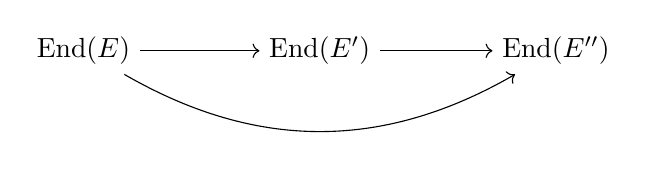
\begin{tikzpicture}
        \node (E1) at (0, 0) {$\End(E)$};
        \node (E2) at (3, 0) {$\End(E')$};
        \node (E3) at (6, 0) {$\End(E'')$};

        \draw [->] (E1) to (E2);
        \draw [->] (E2) to (E3);
        \draw [->] (E1) to [bend right] (E3);
    \end{tikzpicture}
\end{center}
commutes.
\begin{prop}
    Let $E$ be an ordinary Elliptic Curve defined over $k$ and assume that $\Order := \End(E)$ is an order in a quadratic imaginary number field.
    For an ideal $\mathfrak{a} \leq \Order$ define
    \begin{equation*}
        E[\mathfrak{a}] := \bigcap_{a \in \mathfrak{a}} \ker(a)
    \end{equation*}
    Then the map
    \begin{equation*}
        \Cl(\Order) \times \Ell(\Order) \to \Ell(\Order), \quad ([\mathfrak{a}], [E]) \mapsto [E/E[\mathfrak{a}]]
    \end{equation*}
    defines a (well-defined) group action of $\Cl(\Order)$ on $\Ell(\Order)$ (we choose $\mathfrak{a}$ to be an integral ideal representative of the class $[\mathfrak{a}]$)\footnote{Note that for a curve $E'$ that is not $E$, the notation $E'[\mathfrak{a}]$ means $E'[\Phi_*(\mathfrak{a})]$ where $\Phi_*$ is the canonical isomorphism $\End(E) = \Order \to \End(E')$.}.
\end{prop}
\begin{proof}
    First, we show that $\End(E/E[\mathfrak{p}]) \cong \Order$ for an invertible ideal $\mathfrak{p} \leq \Order$.

    Now we show that for (invertible) ideals $\mathfrak{a}, \mathfrak{b} \leq \Order$, we have
    \begin{equation*}
        E/E[\mathfrak{b}\mathfrak{a}] \cong E'/E'[\mathfrak{a}] \quad \text{where $E' = E/E[\mathfrak{b}]$}
    \end{equation*}
    The tricky part here is that we identified the isomorphic endomorphism rings $\End(E)$ and $\End(E')$, but the isomorphism is only on the level of rings (and we also need the kernel of endomorphisms).
    So let's be explicit about which ring we are in.

    Consider the isogenies
    \begin{align*}
        &\phi: E \to E' = E/E[\mathfrak{b}] \quad \text{with kernel $E[\mathfrak{b}]$} \\
        &\psi: E' \to E'/E'[\mathfrak{a}] \quad \text{with kernel $E'[\mathfrak{a}]$}
    \end{align*}
    It suffices to show that $\ker(\psi \circ \phi) = E[\mathfrak{b}\mathfrak{a}]$.

    Consider any $\tau \in \mathfrak{a}$ and let $\tau'$ be the image under the isomorphism $\End(E) \cong \End(E')$.
    Now have that $\tau' \circ \phi = \phi \circ \tau$ (since the isomorphism is $\Phi_*$).
    Hence
    \begin{align*}
        \ker(\psi \circ \phi) =& \phi^{-1}(\ker\psi) = \phi^{-1}(E'[\mathfrak{a}]) = \phi^{-1}\Bigl( \bigcap_{\tau \in \mathfrak{a}} \ker(\tau') \Bigr) \\
        =& \bigcap_{\tau \in \mathfrak{a}} \phi^{-1}(\ker(\tau')) = \bigcap_{\tau \in \mathfrak{a}} \ker(\tau' \circ \phi) = \bigcap_{\tau \in \mathfrak{a}} \ker(\phi \circ \tau) = \bigcap_{\tau \in \mathfrak{a}} \tau^{-1}(\ker\phi) \\
        =& \bigcap_{\tau \in \mathfrak{a}} \tau^{-1}(E[\mathfrak{b}]) = \bigcap_{\tau \in \mathfrak{a}, \ \rho \in \mathfrak{b}} \tau^{-1}(\ker\rho) = \bigcap_{\tau \in \mathfrak{a}, \ \rho \in \mathfrak{b}} \ker(\underbrace{\rho \circ \tau}_{\mathclap{= \rho\tau \in \End(E)}}) = E[\mathfrak{b}\mathfrak{a}]
    \end{align*}
    The claim now follows, since clearly $E/E[(\alpha)] \cong E$ for a principal ideal $(\alpha) \leq \End(E)$.
\end{proof}
\begin{prop}
    This action is faithful (even free?) and transitive.
\end{prop}
\begin{prop}[CSIDH class group action]
    Let $E$ be an Elliptic Curve defined over $k := \F_p$.
    Denote $\Order := \End_k(E)$.
    Then $\Cl(\Order)$ acts on $\Ell_k(\Order)$ via
    \begin{equation*}
        \Cl(\Order) \times \Ell_k(\Order) \to \Ell_k(\Order), \quad ([\mathfrak{a}], E) \mapsto [E/E[\mathfrak{a}]]
    \end{equation*}
\end{prop}
\begin{prop}
    This action is faithful (even free?) and transitive.
\end{prop}
\begin{remark}
    If $E$ is a supersingular Elliptic Curve defined over $k := \F_p$, then $\pi^2 = -p$ and so $\End_k(E) \cong \Z[\sqrt{-p}]$.
    Conversely, if $E$ is ordinary, then $\pi^2 + t \pi + p = 0$ for $t \neq 0$ and so $\End_k(E) \cong \Z[\alpha]$ with $\alpha = \sqrt{t^2/4 - p}$ or $\alpha = 1/2 + \sqrt{t^2/4 - p}$.
    Hence
    \begin{equation*}
        \Ell_k(\Z[\sqrt{-p}]) = \{ E \ | \ \text{$E$ supersingular Elliptic Curve defined over $k = \F_p$} \} / \cong
    \end{equation*}
\end{remark}

\subsection{Summary - Ordinary Elliptic Curves}
\begin{theorem}
    Let $E$ be an ordinary Elliptic Curve defined over $\F_q$.
    Let $\Order := \End(E)$ and $\pi$ be the $q$-th power Frobenius endomorphism of $E$.
    Furthermore, let $t \in \Z$ be the trace of $\pi$.
    Then
    \begin{itemize}
        \item $\Order$ is an order in the quadratic imaginary number field $\mathbb{Q}[\sqrt{D}]$ where $D = t^2 - 4q$.
        Note that $\mathbb{Q}[\sqrt{D}] = \mathbb{Q}[\sqrt{D'}]$ if $D = a^2D'$, and in general $D$ is not square-free.
        \item $\Z[\pi] \subseteq \Order$ (in general no equality).
        \item For an integral ideal $\mathfrak{a} \leq \Order$ such that $p \notdivides [\Order : \mathfrak{a}]$, the isogeny $E \to E/E[\mathfrak{a}]$ has degree $[\Order : \mathfrak{a}]$.
    \end{itemize}
    There is a faithful and transitive group action of $\Cl(\Order)$ on $\Ell(\Order)$ via $[\mathfrak{a}].E = E/E[\mathfrak{a}]$.
\end{theorem}

%\section*{Notes}
%\subsection*{$(d, \epsilon)$-structures}
%Let $p$ be a prime.
%Consider the category $\mathrm{EC}$ defined by
%\begin{align*}
%    \mathrm{Ob}(\mathrm{EC}) &:= \{ \text{$E$ elliptic curve over $\F_{p^2}$} \} \\
%    \mathrm{Hom}_{\mathrm{EC}}(E, E') &:= \{ \text{$\psi: E \to E'$ isogeny} \}
%\end{align*}
%Have a functor
%\begin{align*}
%    \cdot^{(p)}: \mathrm{EC} \ &\to \ \mathrm{EC} \\
%    \text{$E$ defined by $y^2 = x^3 + Ax + B$} \ &\mapsto \ \text{$E'$ defined by $y^2 = x^3 + A^p x + B^p$} \\
%    \left[ \sum_{i, j} a_{ij} x^i y^j : \sum_{i, j} b_{ij} x^i y^j : \sum_{i, j} c_{ij} x^i y^j \right] \ &\mapsto \ \left[ \sum_{i, j} a_{ij}^p x^i y^j : \sum_{i, j} b_{ij}^p x^i y^j : \sum_{i, j} c_{ij}^p x^i y^j \right]
%\end{align*}
%and a functor
%\begin{align*}
%    \hat{\cdot}: \mathrm{EC} \ \to \ \mathrm{EC}^{\mathrm{op}}, \quad E \ \mapsto \ E, \quad \phi \ \mapsto \ \hat{\phi}
%\end{align*}
%$(d, \epsilon)$-structures and their isogenies are given by the category $\mathcal{C}$ defined by
%\begin{align*}
%    \mathrm{Ob}(\mathcal{C}) &:= \{ (E, \psi) \ | \ E \in \mathrm{EC}, \ \psi: E \to E^{(p)} \ \text{degree $d$ isogeny}, \ \hat{\psi} = \epsilon\psi^{(p)} \} \\
%    \mathrm{Hom}_{\mathcal{C}}((E, \psi), (E', \psi')) &:= \{ \phi: E \to E' \ | \ \psi' \circ \phi = \phi^{(p)} \circ \psi \}
%\end{align*}
%
%\subsection*{Endomorphism Ring}
%Consider a supersingular curve $E$ defined over $\F_q$ and $\pi = \pi_q$ the Frobenius endomorphism.
%Then
%\begin{equation*}
%    \mathrm{End}(E) \neq \Z[\pi] = \underbrace{\mathrm{End}_{\F_q}(E)}_{\mathclap{\text{endomorphisms defined over $\F_q$}}}
%\end{equation*}
%and $\Z[\pi]$ is a commutative ring (either $\Z$ or an order in an imaginary quadratic number field).
%In particular, there is an endomorphism (I believe even automorphism) $\psi$ not defined over $\F_q$ such that $\psi \notin \Z[\pi]$ and $\pi, \psi$ do not commute.
\end{document}